\documentclass[11pt]{article}
\usepackage[margin=1in]{geometry}
\usepackage{graphicx}
\usepackage{booktabs}
\usepackage{array}
\usepackage{hyperref}
\hypersetup{colorlinks=true, linkcolor=black, citecolor=black, urlcolor=black}
\usepackage{titlesec}
\usepackage{needspace}
\titlespacing*{\section}{0pt}{10pt}{3pt}
\titlespacing*{\subsection}{0pt}{8pt}{3pt}
\setlength{\parindent}{0pt}
\setlength{\parskip}{5pt}

\title{\vspace{-1.5em}Social Influence Prediction: GNN-Based Modeling of Peer Behavior}
\author{}
\date{}

\begin{document}
\maketitle
\vspace{-3em}
{\small Problem statement DSAI\_PS\_1 --- codebase + trained weights + this report}

\section*{1. Problem}
Given a social graph, an ego user $v$, and the binary action state of $v$'s neighbors, predict the probability that $v$ performs the same action (ad view, product adoption, repost). We treat this as node-level binary classification, encoding $v$'s local neighborhood with a graph neural network instead of scoring $v$ in isolation, on the premise that what a user's neighbors do carries predictive signal beyond $v$'s own attributes.

\section*{2. Data}
The datasets named in the problem statement (OAG / Digg / Weibo, from the DeepInf paper) were not accessible in the time we had, so we used the second option the problem statement itself allows: a synthetic graph with simulated cascades. We built a 1200-node Barabasi-Albert graph (scale-free, so a few hub users and many low-degree users, matching real social network structure) and ran six independent-cascade simulations over it (15 seed users each, $p=0.06$ transmission probability per edge per step). Every node gets an activation time or never activates; the label $y$ is whether it was ever activated. Positive rate came out to 21.5\%.

\section*{3. Pipeline}
Every stage below matches the problem statement's pipeline section. All models share the same encoder and head implementation, so the comparisons in section 5 isolate the one thing each row is testing.

\begin{center}
\begin{tabular}{@{}p{3.6cm}p{10.4cm}@{}}
\toprule
\textbf{Stage} & \textbf{Implementation} \\
\midrule
(a) Ego network sampling & Truncated BFS, fixed $k$-hop radius, max 20 nodes, zero-padded for batching \\
(b) Graph encoding & 2-layer GCN, symmetric-normalized adjacency, self-loops (Kipf and Welling) \\
(c) Instance normalization & Per-instance, per-channel normalization across sampled nodes, padding masked out \\
(d) Handcrafted features & Degree, clustering coefficient, active-neighbor count, influence ratio, active fraction, demographics \\
(e) Prediction head & 2-layer MLP, sigmoid output \\
(f) Training & Binary cross-entropy, end-to-end backprop through encoder + head, Adam with weight decay \\
\bottomrule
\end{tabular}
\end{center}

\section*{4. Baselines}
Four models, matching the comparison table in the problem statement: Logistic Regression on handcrafted features only; DeepWalk-style embeddings (32-d, computed via NetMF, a closed-form equivalent of DeepWalk's skip-gram objective) with an MLP on top; a Plain GCN with no handcrafted-feature fusion; and the Full model, which is the GCN encoder with handcrafted features concatenated in before the head.

\section*{5. Results}
\begin{center}
\begin{tabular}{@{}lrrrr@{}}
\toprule
\textbf{Model} & \textbf{AUC-ROC} & \textbf{F1} & \textbf{Precision} & \textbf{Recall} \\
\midrule
Logistic Regression & 0.666 & 0.426 & 1.000 & 0.270 \\
DeepWalk + MLP & 0.662 & 0.000 & 0.000 & 0.000 \\
Plain GCN & 0.807 & 0.604 & 1.000 & 0.432 \\
Full model (proposed) & 0.835 & 0.538 & 0.933 & 0.378 \\
Full model, no instance norm & 0.819 & 0.607 & 0.895 & 0.459 \\
\bottomrule
\end{tabular}
\end{center}

All numbers are on a held-out test split (180 users, 15\% of the graph) not touched during training or model selection. Both GCN-based models clearly beat the two non-graph baselines by 14--17 points of AUC. That's the central claim the problem statement sets out to test, and it holds by a wide margin. DeepWalk+MLP tracks Logistic Regression almost exactly (0.662 vs 0.666 AUC) and its F1 collapsed to 0 at the default threshold: the embeddings encode graph position, not neighbors' current action state, and graph position isn't what this task actually needs. Handcrafted fusion is a modest, not decisive, win here: 0.835 vs 0.807 AUC, but lower F1 and recall than Plain GCN. On this synthetic graph two of the handcrafted features are algebraically identical (active-neighbor ratio and fraction of active neighbors both reduce to active/degree), so there isn't much independent signal left for fusion to add. Instance normalization raises AUC (0.835 vs 0.819) at some cost to recall, consistent with it changing decision-boundary shape without changing what the model has learned.

\section*{6. Loss curves}

\begin{center}
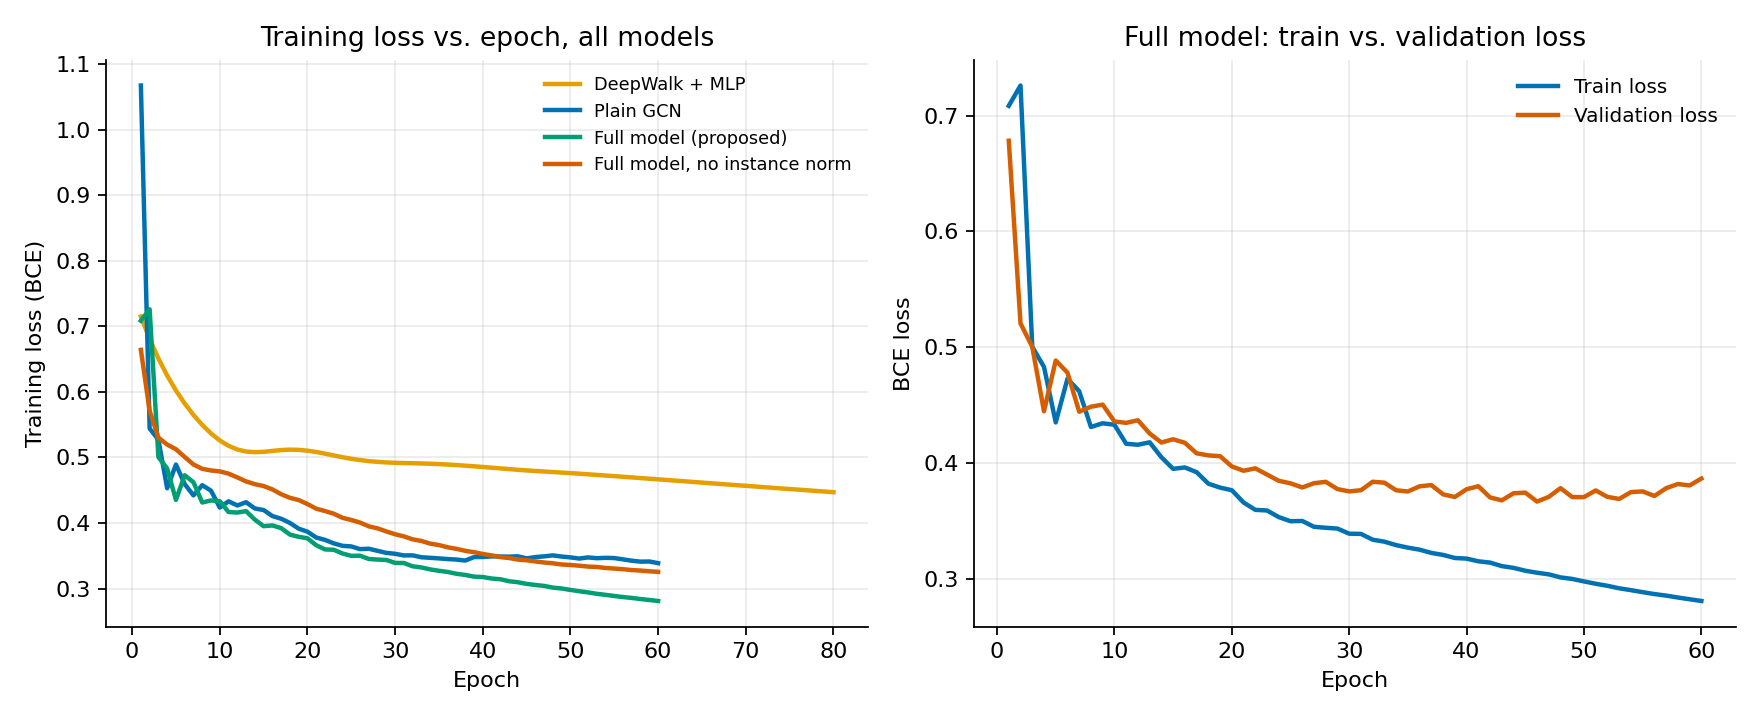
\includegraphics[width=0.92\textwidth]{outputs/loss_vs_epoch.png}
\end{center}

Left: training loss for all four trained models, overlaid. Right: train vs validation loss for the full model specifically.

The GCN-based models converge to a visibly lower loss than DeepWalk+MLP, matching the AUC gap. For the full model, train and validation loss track together for about the first 15 epochs, then validation loss flattens around 0.37--0.38 while training loss keeps falling toward 0.28. That's mild overfitting past epoch $\sim$25, and worth mentioning rather than just reporting the final-epoch number.

\section*{7. Ablations}
Sensitivity to ego-network radius $k$, full model, same train/val/test split:

\begin{center}
\begin{tabular}{@{}lrrrr@{}}
\toprule
\textbf{$k$-hop radius} & \textbf{AUC-ROC} & \textbf{F1} & \textbf{Precision} & \textbf{Recall} \\
\midrule
$k=1$ & 0.707 & 0.462 & 0.800 & 0.324 \\
$k=2$ & 0.801 & 0.618 & 0.944 & 0.459 \\
$k=3$ & 0.865 & 0.643 & 0.947 & 0.486 \\
\bottomrule
\end{tabular}
\end{center}

AUC rises monotonically with $k$ (0.707 to 0.865 from 1-hop to 3-hop), with no sign of saturating by $k=3$. That says 2-hop information (what a user's friends-of-friends have done) is genuinely predictive here and not just noise the model has to filter past, which tracks with how far the cascade simulation itself propagates per step.

\section*{8. Recommendation}
Use the full model (GCN + handcrafted fusion + instance norm), but extend the $k$-sweep to $k=4,5$ before finalizing since AUC was still climbing at $k=3$ and hadn't plateaued. Report the handcrafted-fusion gain as modest rather than decisive on this synthetic dataset, and re-check it on the real DeepInf datasets (OAG/Digg/Weibo) where non-graph user attributes should carry more independent signal than the synthetic demographics used here, which were generated independently of the cascade process and so carry none by construction.

\end{document}
